

\documentclass[11pt,compress,t,notes=noshow, xcolor=table]{beamer}
\usepackage[]{graphicx}\usepackage[]{color}
% maxwidth is the original width if it is less than linewidth
% otherwise use linewidth (to make sure the graphics do not exceed the margin)
\makeatletter
\def\maxwidth{ %
  \ifdim\Gin@nat@width>\linewidth
    \linewidth
  \else
    \Gin@nat@width
  \fi
}
\makeatother

\newcommand{\citebutton}[2]{%
\beamergotobutton{\href{#2}{#1}}%
}

\newcommand{\blu}[1]{\textcolor{blue}{#1}}
\newcommand{\org}[1]{\textcolor{orange}{#1}}
\newcommand{\ques}{\textbf{\textcolor{red}{Question:  }}}
\newcommand{\questionssofar}{\begin{frame}\frametitle{Any questions?}\end{frame}}

\newcommand\warning{%
 \makebox[1.4em][c]{%
 \makebox[0pt][c]{\raisebox{.1em}{\scriptsize!}}%
 \makebox[0pt][c]{\color{red}\normalsize$\bigtriangleup$}}}%

\definecolor{fgcolor}{rgb}{0.345, 0.345, 0.345}
\newcommand{\hlnum}[1]{\textcolor[rgb]{0.686,0.059,0.569}{#1}}%
\newcommand{\hlstr}[1]{\textcolor[rgb]{0.192,0.494,0.8}{#1}}%
\newcommand{\hlcom}[1]{\textcolor[rgb]{0.678,0.584,0.686}{\textit{#1}}}%
\newcommand{\hlopt}[1]{\textcolor[rgb]{0,0,0}{#1}}%
\newcommand{\hlstd}[1]{\textcolor[rgb]{0.345,0.345,0.345}{#1}}%
\newcommand{\hlkwa}[1]{\textcolor[rgb]{0.161,0.373,0.58}{\textbf{#1}}}%
\newcommand{\hlkwb}[1]{\textcolor[rgb]{0.69,0.353,0.396}{#1}}%
\newcommand{\hlkwc}[1]{\textcolor[rgb]{0.333,0.667,0.333}{#1}}%
\newcommand{\hlkwd}[1]{\textcolor[rgb]{0.737,0.353,0.396}{\textbf{#1}}}%
\let\hlipl\hlkwb

\usepackage{framed}
\makeatletter
\newenvironment{kframe}{%
 \def\at@end@of@kframe{}%
 \ifinner\ifhmode%
  \def\at@end@of@kframe{\end{minipage}}%
  \begin{minipage}{\columnwidth}%
 \fi\fi%
 \def\FrameCommand##1{\hskip\@totalleftmargin \hskip-\fboxsep
 \colorbox{shadecolor}{##1}\hskip-\fboxsep
     % There is no \\@totalrightmargin, so:
     \hskip-\linewidth \hskip-\@totalleftmargin \hskip\columnwidth}%
 \MakeFramed {\advance\hsize-\width
   \@totalleftmargin\z@ \linewidth\hsize
   \@setminipage}}%
 {\par\unskip\endMakeFramed%
 \at@end@of@kframe}
\makeatother

\definecolor{shadecolor}{rgb}{.97, .97, .97}
\definecolor{messagecolor}{rgb}{0, 0, 0}
\definecolor{warningcolor}{rgb}{1, 0, 1}
\definecolor{errorcolor}{rgb}{1, 0, 0}
\newenvironment{knitrout}{}{} % an empty environment to be redefined in TeX

\usepackage{alltt}
\newcommand{\SweaveOpts}[1]{}  % do not interfere with LaTeX
\newcommand{\SweaveInput}[1]{} % because they are not real TeX commands
\newcommand{\Sexpr}[1]{}       % will only be parsed by R
\newcommand{\xmark}{\ding{55}}%


\usepackage[english]{babel}
\usepackage[utf8]{inputenc}

\usepackage{dsfont}
\usepackage{verbatim}
\usepackage{amsmath}
\usepackage{amsfonts}
\usepackage{amssymb}
\usepackage{bm}
\usepackage{csquotes}
\usepackage{multirow}
\usepackage{longtable}
\usepackage{booktabs}
\usepackage{enumerate}
\usepackage[absolute,overlay]{textpos}
\usepackage{psfrag}
\usepackage{algorithm}
\usepackage{algpseudocode}
\usepackage{eqnarray}
\usepackage{arydshln}
\usepackage{tabularx}
\usepackage{placeins}
\usepackage{tikz}
\usepackage{setspace}
\usepackage{colortbl}
\usepackage{mathtools}
\usepackage{wrapfig}
\usepackage{bm}
\usepackage{amsmath}
\usepackage{pifont}

\usetikzlibrary{shapes.multipart,shapes,arrows,automata,positioning,calc,chains,trees, shadows}
\tikzset{
  %Define standard arrow tip
  >=stealth',
  %Define style for boxes
  punkt/.style={
    rectangle,
    rounded corners,
    draw=black, very thick,
    text width=6.5em,
    minimum height=2em,
    text centered},
  % Define arrow style
  pil/.style={
    ->,
    thick,
    shorten <=2pt,
    shorten >=2pt,}
}

\tikzstyle{vec}=[draw, rectangle, fill = white, minimum width=5mm, minimum height=1cm, inner sep = 2pt]

\usepackage{subfig}

% Defines macros and environments
\usepackage{../../style/lmu-lecture}


\let\code=\texttt
\let\proglang=\textsf

\setkeys{Gin}{width=0.9\textwidth}

\setbeamertemplate{frametitle}{\expandafter\uppercase\expandafter\insertframetitle}

\usepackage{bbm}
% basic latex stuff
\newcommand{\pkg}[1]{{\fontseries{b}\selectfont #1}} %fontstyle for R packages
\newcommand{\lz}{\vspace{0.5cm}} %vertical space
\newcommand{\dlz}{\vspace{1cm}} %double vertical space
\newcommand{\oneliner}[1] % Oneliner for important statements
{\begin{block}{}\begin{center}\begin{Large}#1\end{Large}\end{center}\end{block}}


%new environments
\newenvironment{vbframe}  %frame with breaks and verbatim
{
 \begin{frame}[containsverbatim,allowframebreaks]
}
{
\end{frame}
}

\newenvironment{vframe}  %frame with verbatim without breaks (to avoid numbering one slided frames)
{
 \begin{frame}[containsverbatim]
}
{
\end{frame}
}

\newenvironment{blocki}[1]   % itemize block
{
 \begin{block}{#1}\begin{itemize}
}
{
\end{itemize}\end{block}
}

\newenvironment{fragileframe}[2]{  %fragile frame with framebreaks
\begin{frame}[allowframebreaks, fragile, environment = fragileframe]
\frametitle{#1}
#2}
{\end{frame}}


\newcommand{\myframe}[2]{  %short for frame with framebreaks
\begin{frame}[allowframebreaks]
\frametitle{#1}
#2
\end{frame}}

\newcommand{\remark}[1]{
  \textbf{Remark:} #1
}


\newenvironment{deleteframe}
{
\begingroup
\usebackgroundtemplate{
\includegraphics[width=\paperwidth,height=\paperheight]{../style/color/red.png}}
 \begin{frame}
}
{
\end{frame}
\endgroup
}
\newenvironment{simplifyframe}
{
\begingroup
\usebackgroundtemplate{
\includegraphics[width=\paperwidth,height=\paperheight]{../style/color/yellow.png}}
 \begin{frame}
}
{
\end{frame}
\endgroup
}\newenvironment{draftframe}
{
\begingroup
\usebackgroundtemplate{
\includegraphics[width=\paperwidth,height=\paperheight]{../style/color/green.jpg}}
 \begin{frame}
}
{
\end{frame}
\endgroup
}
% https://tex.stackexchange.com/a/261480: textcolor that works in mathmode
\makeatletter
\renewcommand*{\@textcolor}[3]{%
  \protect\leavevmode
  \begingroup
    \color#1{#2}#3%
  \endgroup
}
\makeatother





\usepackage{xspace}
\input{../../latex-math/basic-math.tex}
\input{../../latex-math/basic-ml.tex}

\def\cotpfull{chain-of-thought prompting\xspace}
\def\cotp{COT-P\xspace}

%\newcommand{\titlefigure}{figure/gpt_sq.png}
\newcommand{\learninggoals}{
\item illustrate \cotpfull and point out the benefits it brings to LLMs
\item illustrate tree-of-thought and point out the benefits it brings to LLMs 
}

\definecolor{texblue}{rgb}{0, 0, 1}
\def\myblue#1{\textcolor{texblue}{#1}}

\title{\cotpfull}
% \author{}
\institute{\href{https://slds-lmu.github.io/lecture_dl4nlp/}{slds-lmu.github.io/lecture\_dl4nlp}}
\date{}

\begin{document}
\lecturechapter{Large Language Models (LLMs)}
\lecture{Deep Learning for NLP}

% ------------------------------------------------------------------------------ 

\begin{vbframe}{\cotpfull motivation}

\vfill

How to boost the reasoning capabilities of LLMs? \citebutton{Wei et al., 2021}{https://arxiv.org/abs/2109.01652}

\begin{itemize}
\item Use formal approaches, e.g., logic, symbolic reasoning
    \begin{itemize}
    \item Example: \citebutton{BeliefBank}{https://arxiv.org/abs/2109.14723}
\item Difficult to train and deploy, not widely used
    \end{itemize}
\item Standard few-shot learning via prompting works for many tasks
    \begin{itemize}
    \item Still, it works poorly for many tasks that require reasoning
    \end{itemize}
\item \cotp
    \begin{itemize}
    \item A new form of few-shot prompting
    \item Each ``training example'' has the form <input, \textit{chain of thought}, output>
    \item chain of thought:\\ series of reasoning steps that
    lead to the final answer
    \item applications: complex, commonsense, symbolic
    reasoning tasks etc
    \end{itemize}

\end{itemize}

\vfill

\end{vbframe}

\begin{frame}{Neurosymbolic approach\\ (currently
    infrequently used)}

\vfill
	
	\begin{figure}
		\centering
		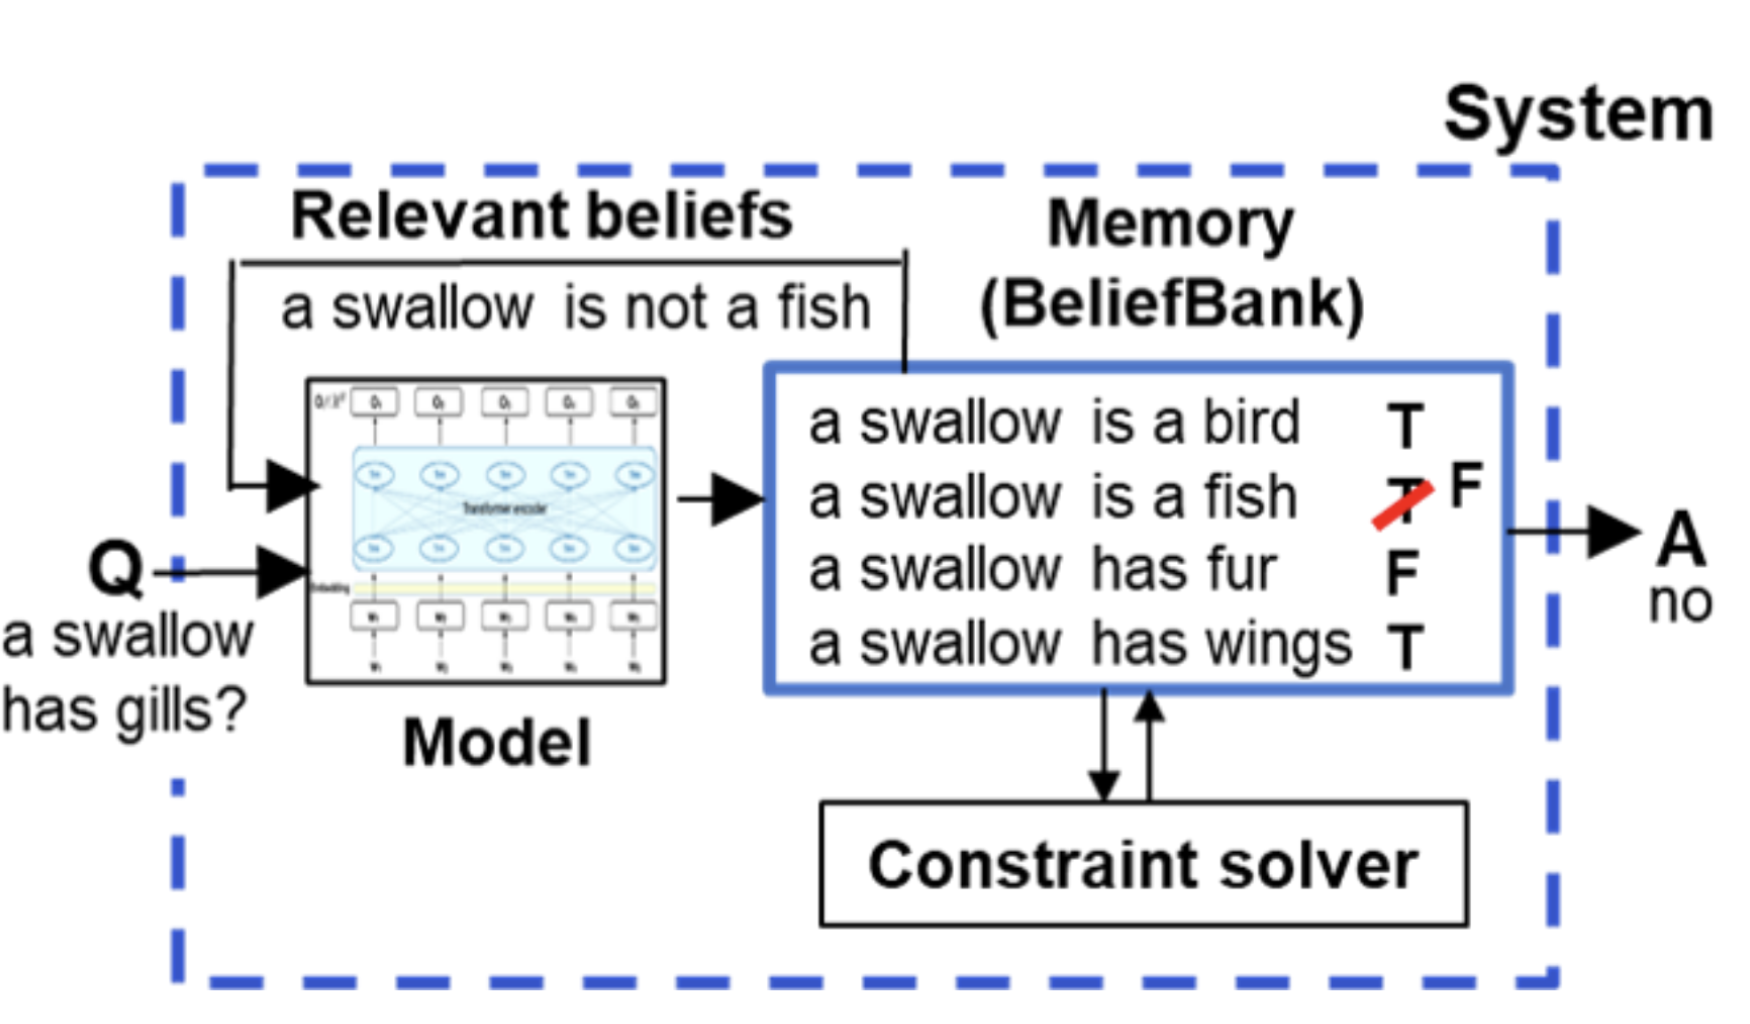
\includegraphics[height = 6cm]{figure/beliefbank} 
	\end{figure}

\vfill

\end{frame}


\begin{frame}{LLMs not good at reasoning tasks}

\vfill
	
	\begin{figure}
		\centering
		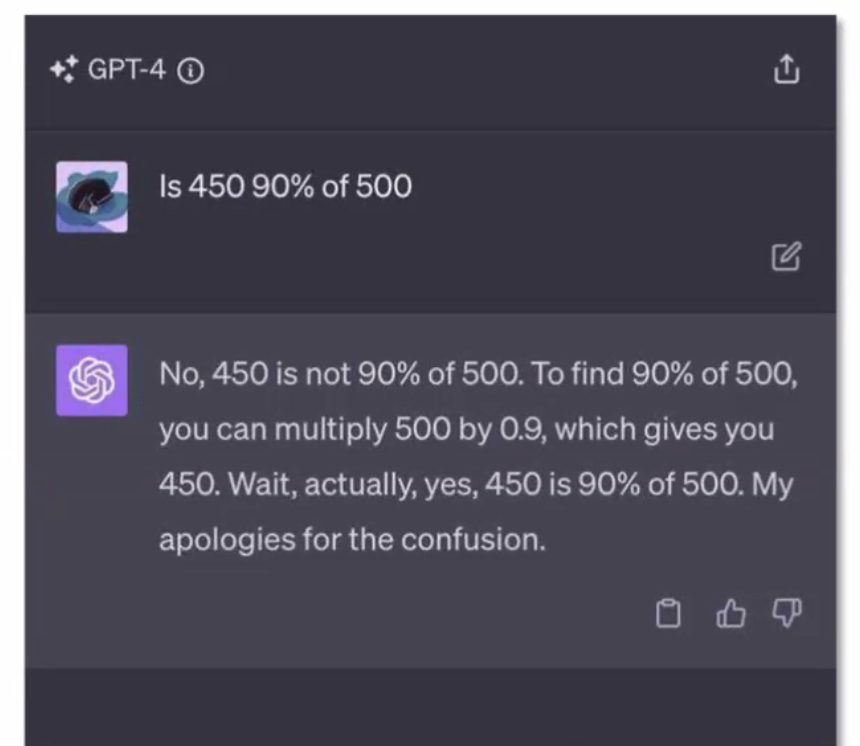
\includegraphics[height = 6cm]{figure/is450,90,of,500} 
	\end{figure}

\ques What is the problem here?
% left-to-right next-token prediction

\vfill

\end{frame}


% ------------------------------------------------------------------------------ 

\begin{vbframe}{\cotpfull paradigm}

\vfill

%\textbf{\cotp enables LLMs to tackle complex arithmetic, commonsense and symbolic reasoning tasks.}

\begin{figure}
    \centering
    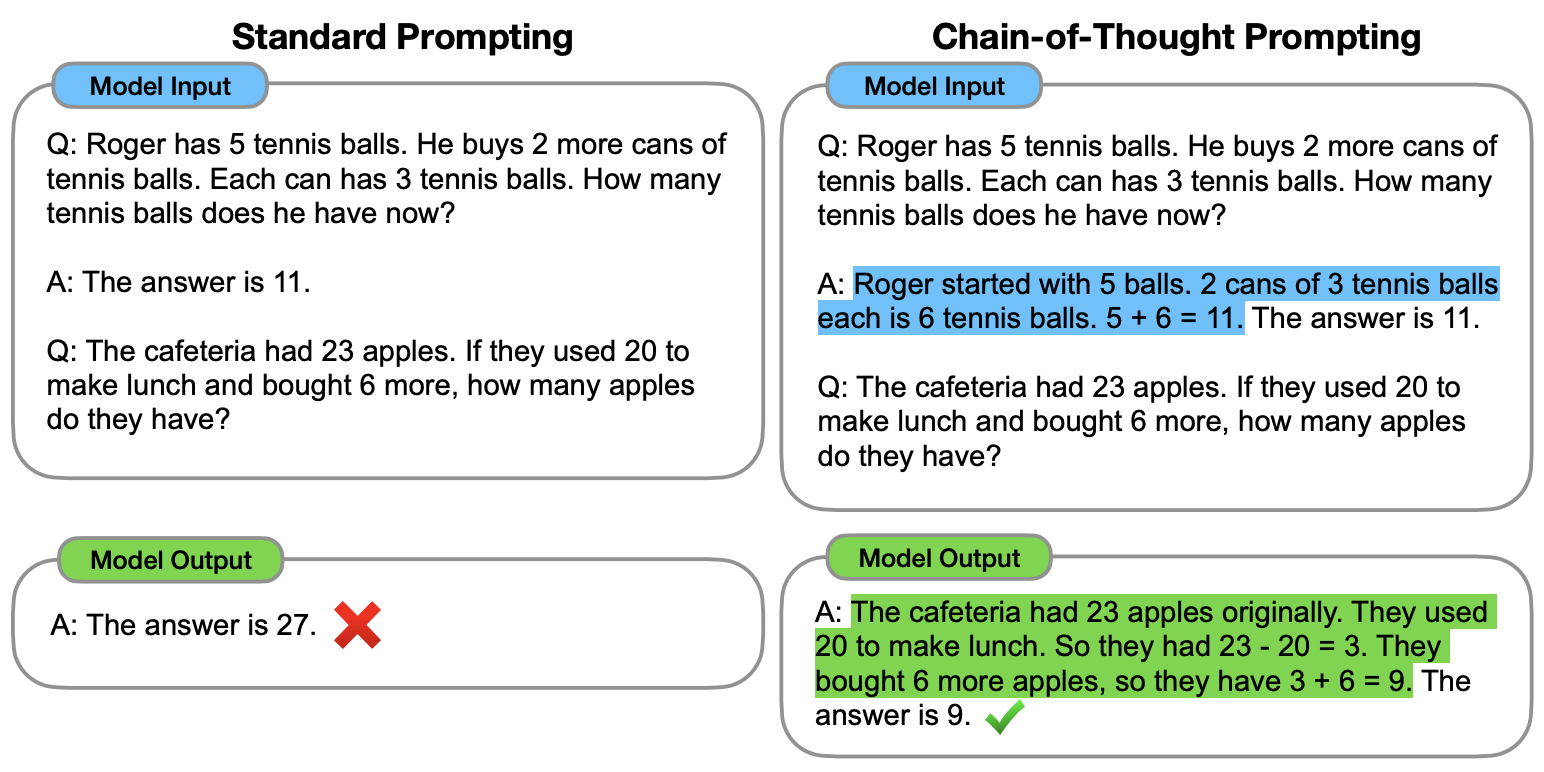
\includegraphics{figure/chain_of_thought.png}\\
    \citebutton{Source: Wei et al., 2022}{https://arxiv.org/pdf/2201.11903.pdf}
\end{figure}

\vfill

\end{vbframe}

% ------------------------------------------------------------------------------ 

\begin{vbframe}{\cotpfull paradigm}

\begin{figure}
    \centering
    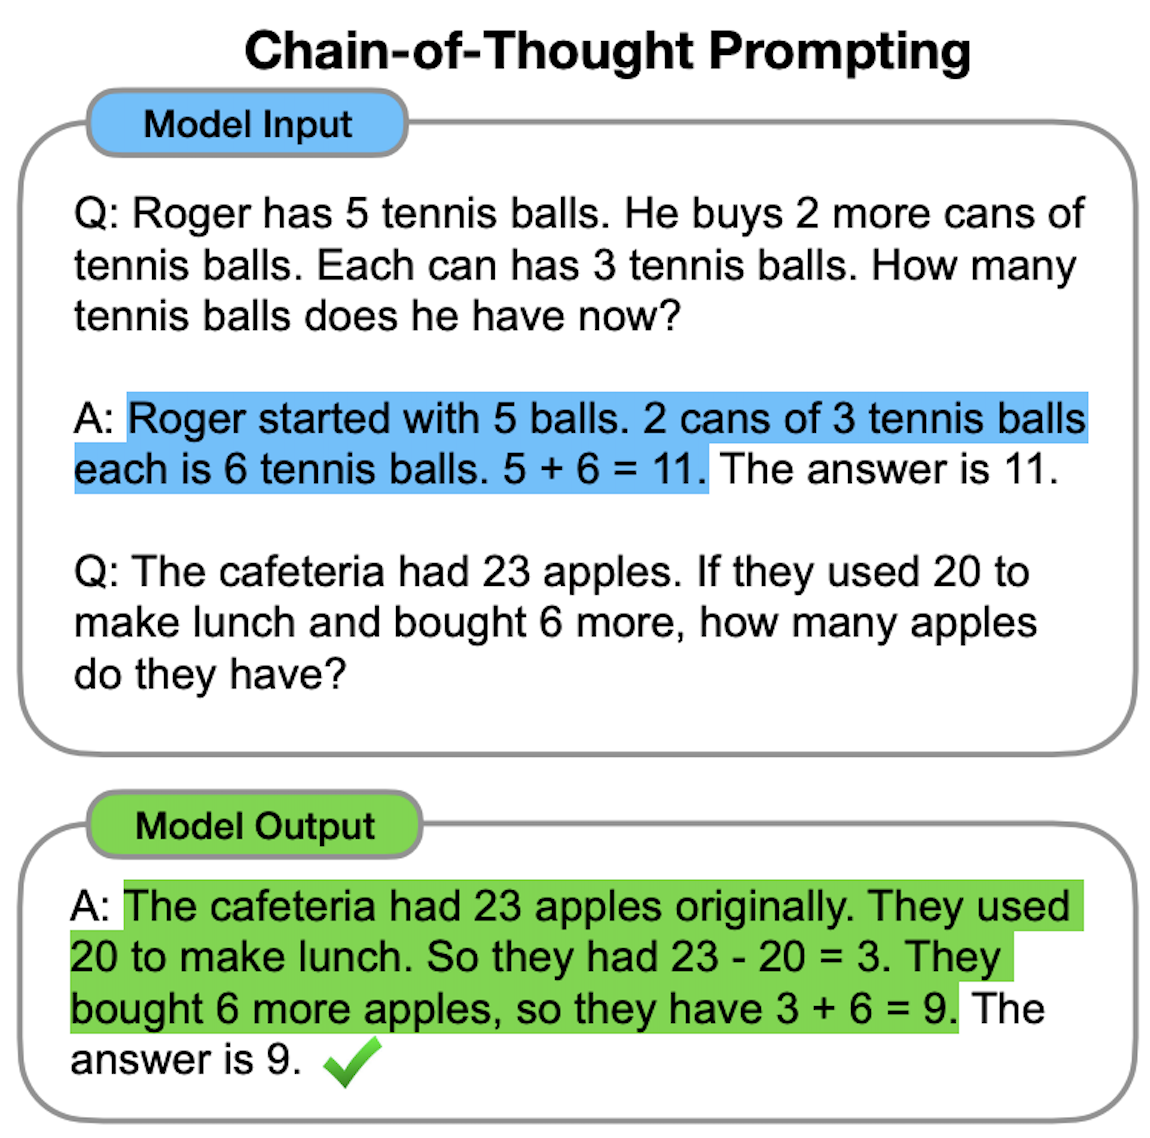
\includegraphics[height=7cm]{figure/chain_of_thought2.png}
\end{figure}

\end{vbframe}

% ------------------------------------------------------------------------------


\begin{vbframe}{Benefits of \cotpfull}

\vfill

\begin{itemize}
    \item Decompose multi-step problems and thus allocate more compute to problems requiring more reasoning steps
    \item By describing the reasoning, interpretability is increased. It provides the possibility to observe where reasoning went wrong
    \item It is closer to how humans solve tasks using language
    \item Language models, if
given a well designed chain-of-thought prompt, can
    solve problems they otherwise would not be able to solve.
\end{itemize}

\vfill

\end{vbframe}


% ------------------------------------------------------------------------------

\begin{vbframe}{Examples of \cotpfull}

\vfill

\textbf{Examples of $<$input, chain of thought, output$>$ triples for  commonsense and symbolic reasoning}

    \citebutton{Source: Wei et al., 2022}{https://arxiv.org/pdf/2201.11903.pdf}

THE FEW SHOTS (TRAINING EXAMPLES) ARE OMITTED FROM THESE
EXAMPLES TO SAVE SPACE, BUT THIS IS CHAIN OF THOUGHT
PROMPTING, THAT IS, THE MODEL IS PROMPTED WITH EXAMPLES OF
CHAIN OF THOUGHT REASONING.


\vfill

\end{vbframe}

% ------------------------------------------------------------------------------

\begin{vbframe}{Examples}

\vfill

\begin{figure}
    \centering
    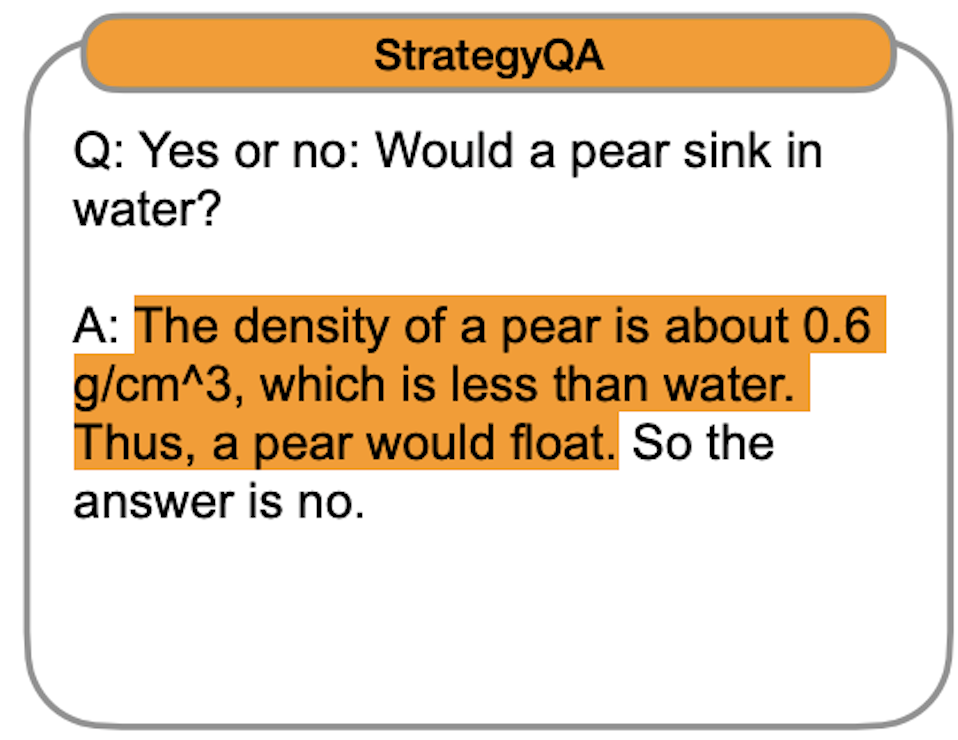
\includegraphics[height=7cm]{figure/cotex1.png}
\end{figure}

\vfill

\end{vbframe}

\begin{vbframe}{Examples}

\vfill

\begin{figure}
    \centering
    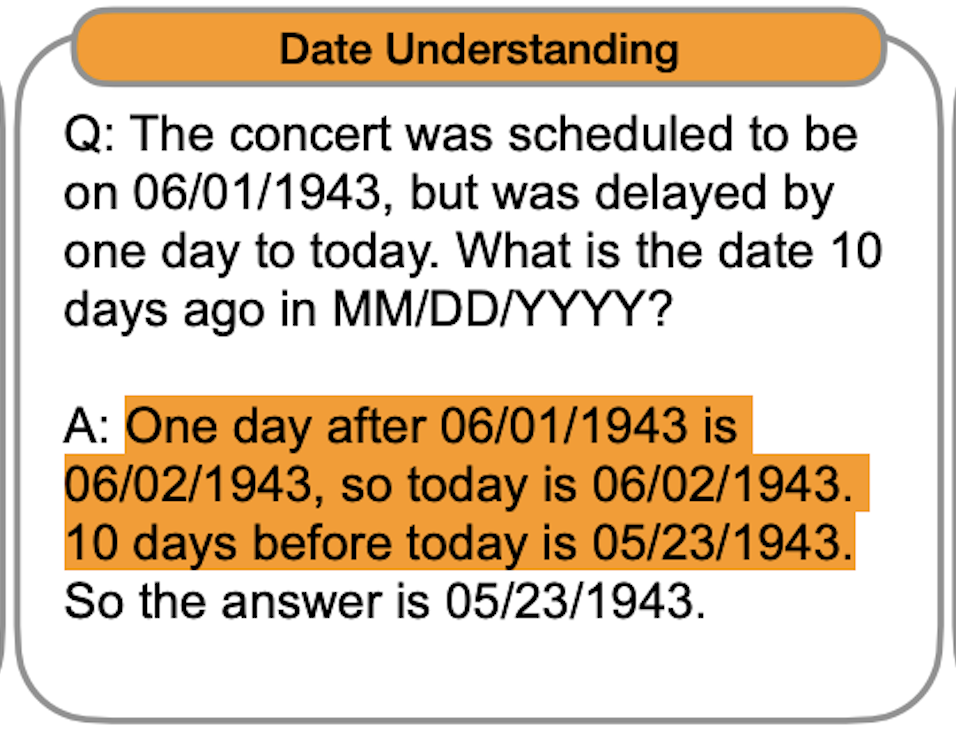
\includegraphics[height=7cm]{figure/cotex2.png}
\end{figure}

\vfill

\end{vbframe}

\begin{vbframe}{Examples}

\vfill

\begin{figure}
    \centering
    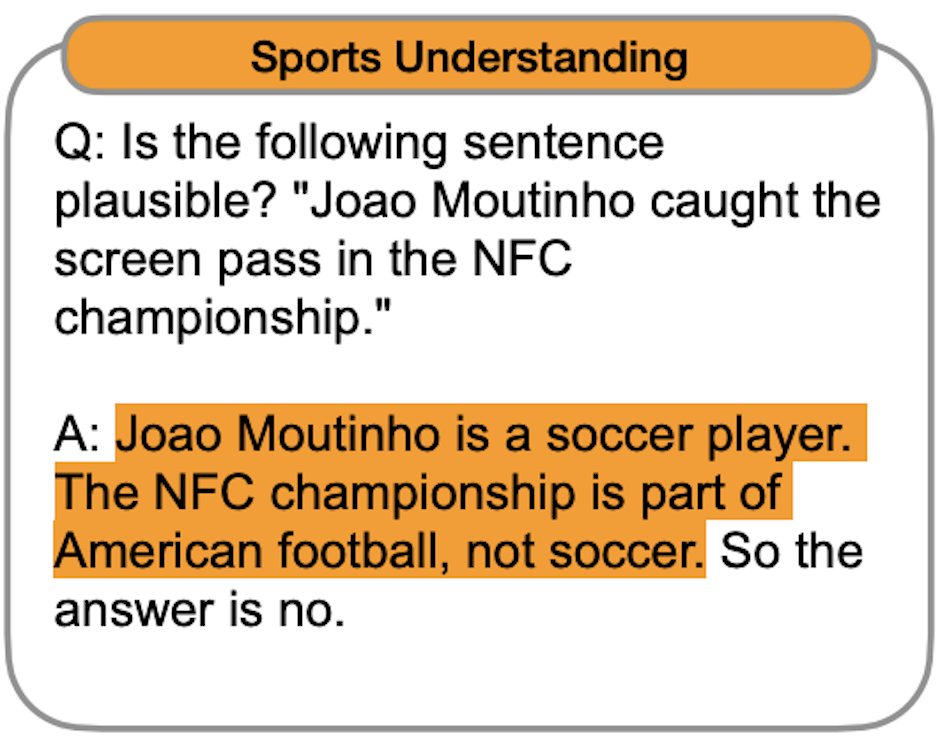
\includegraphics[height=7cm]{figure/cotex3.png}
\end{figure}

\vfill

\end{vbframe}

\begin{vbframe}{Examples}

\vfill

\begin{figure}
    \centering
    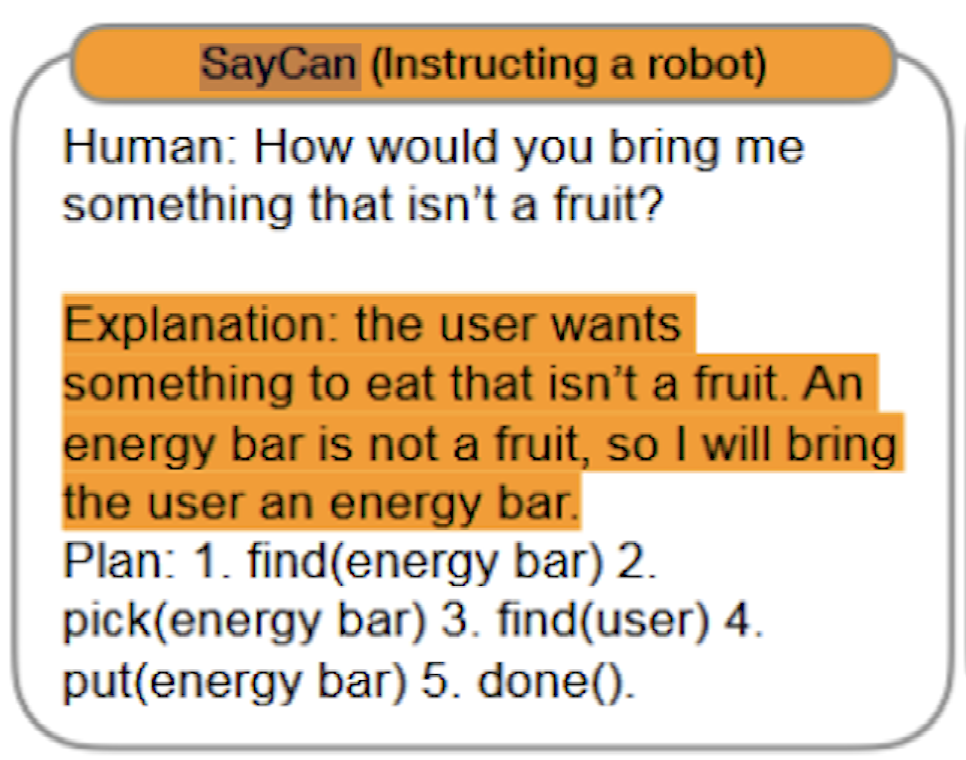
\includegraphics[height=7cm]{figure/cotex4.png}
\end{figure}

\vfill

\end{vbframe}

\begin{vbframe}{Examples}

\vfill

\begin{figure}
    \centering
    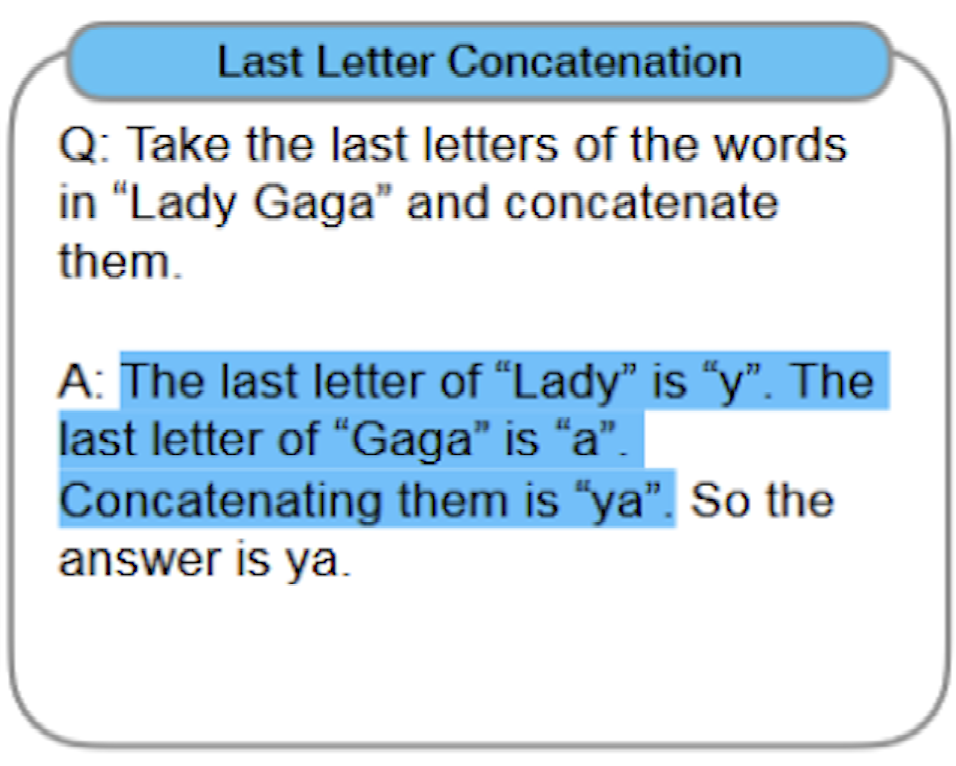
\includegraphics[height=7cm]{figure/cotex5.png}
\end{figure}

\vfill

\end{vbframe}

\begin{vbframe}{Examples}

\vfill

\begin{figure}
    \centering
    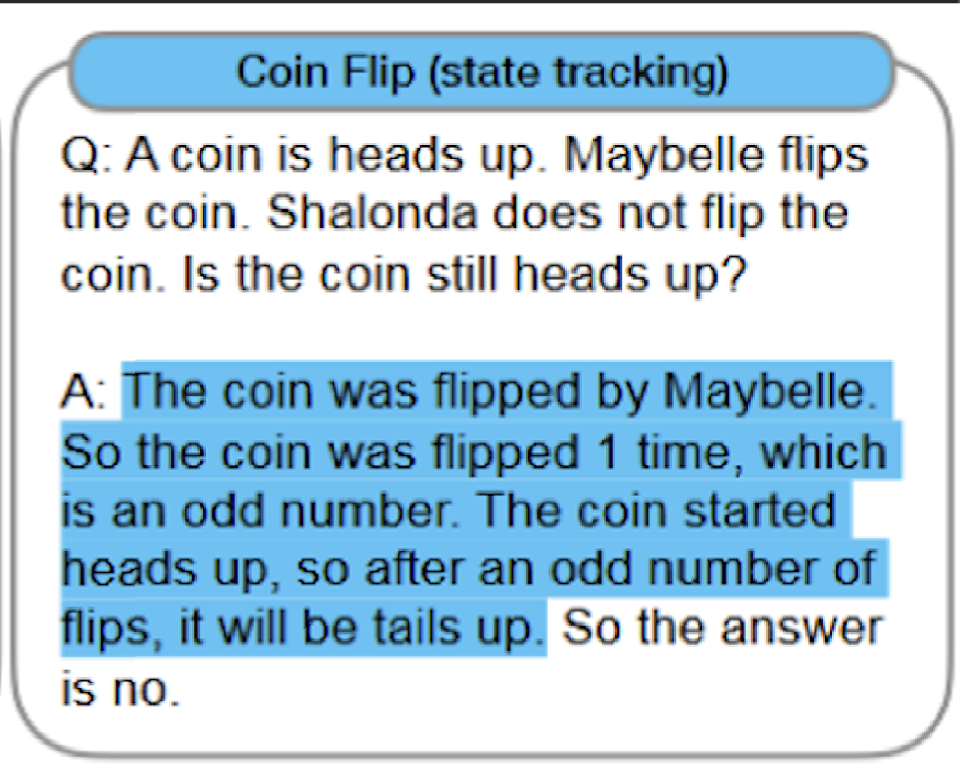
\includegraphics[height=7cm]{figure/cotex6.png}
\end{figure}

\vfill

\end{vbframe}

% ------------------------------------------------------------------------------

\begin{vbframe}{\cotp improves arithmetic}

\vfill
	
	\begin{figure}
		\centering
		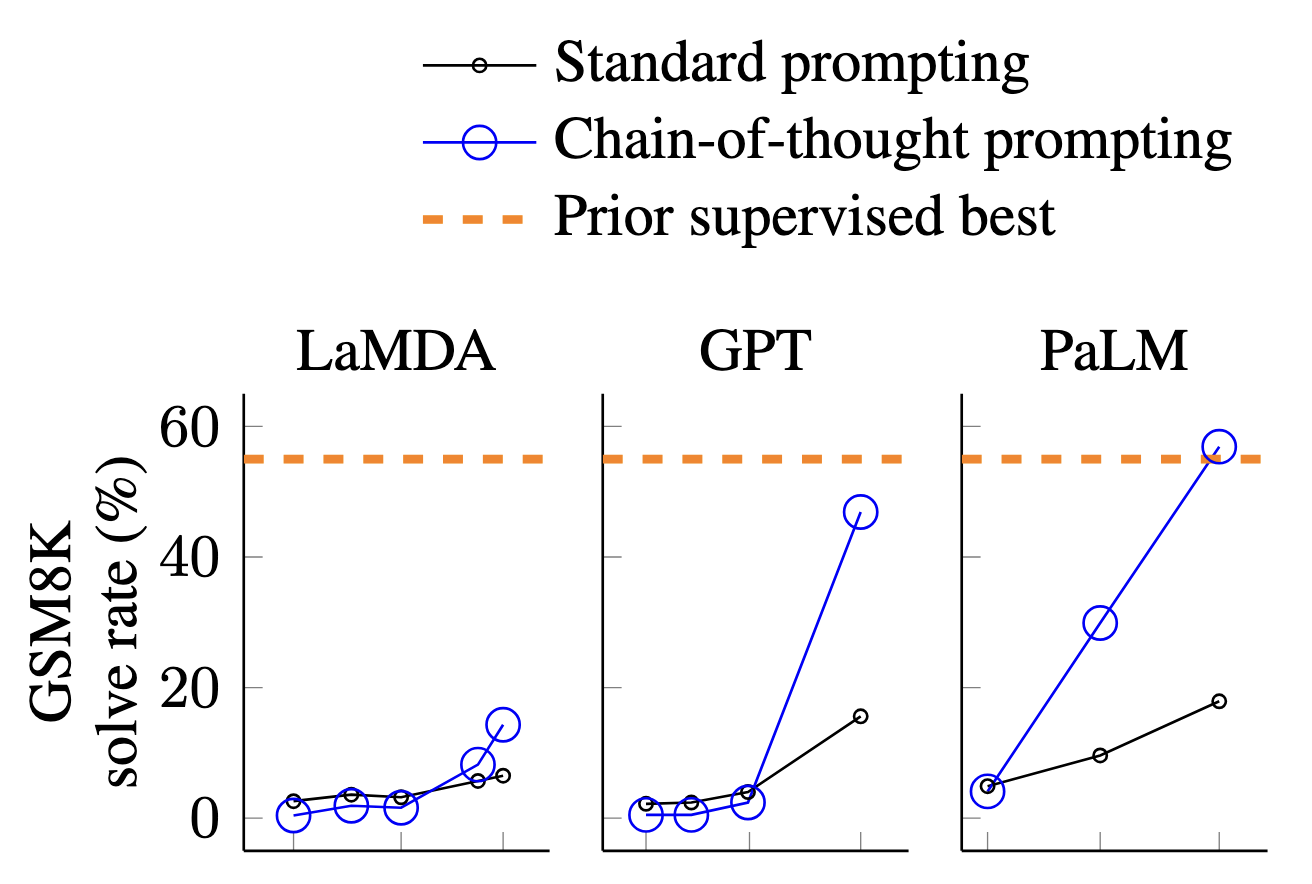
\includegraphics[height = 6cm]{figure/cotperformance} 
	\end{figure}

\vfill

\end{vbframe}


\begin{vbframe}{\cotp improves arithmetic}

%\vfill

SVAMP: math word problems with varying structures; MAWPS:
repository unifying math problems from different sources;
    \citebutton{Source: Wei et al., 2022}{https://arxiv.org/pdf/2201.11903.pdf}

\begin{figure}
    \centering
    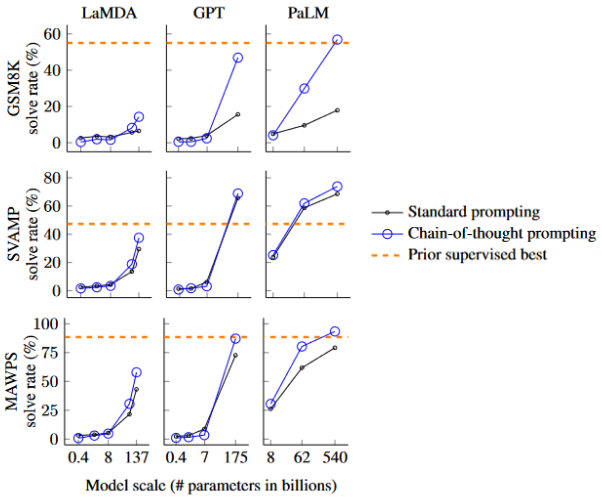
\includegraphics[width=0.5\textwidth]{figure/cot_performance1.png}
\end{figure}

%\vfill

\end{vbframe}

% ------------------------------------------------------------------------------

\begin{vbframe}{\cotp improves commonsense}

\vfill

CSQA: Contains around 200K dialogs with a total of 1.6M
turns. Further, unlike existing large scale QA datasets
which contain simple questions that can be answered from a
single tuple, the questions in the dialogs require a larger
subgraph of the KG. 


\begin{figure}
    \centering
    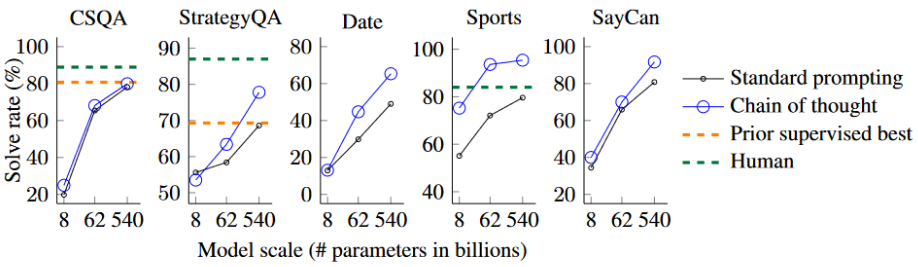
\includegraphics{figure/cot_performance2.png}\\
    \citebutton{Source: Wei et al., 2022}{https://arxiv.org/pdf/2201.11903.pdf}
\end{figure}

\vfill

\end{vbframe}

% ------------------------------------------------------------------------------ 

\begin{vbframe}{tree-of-thought: motivation}

\vfill

\begin{itemize}
\item The token-level and left-to-right decisions of the autoregressive mechanism pose a limitation for:
    \begin{itemize}
    \item Tasks where initial decisions play a pivotal role
    \item Tasks requiring exploration or strategic lookahead
    \end{itemize}
\item Strategy to solve those:
    \begin{itemize}
    \item Maintain and explore diverse alternatives instead of just picking one
    \item Evaluate current status and look ahead or backtrack to make global decisions
    \end{itemize}

\end{itemize}

\vfill

\end{vbframe}

% ------------------------------------------------------------------------------

\begin{vbframe}{Tree-of-thought: prompting paradigm}

\vfill

Schematic illustrating three approaches to problem solving
with LLMs. Rectangle box = \textit{thought} = a coherent language sequence serving as an intermediate step in problem solving.

\begin{figure}
    \centering
    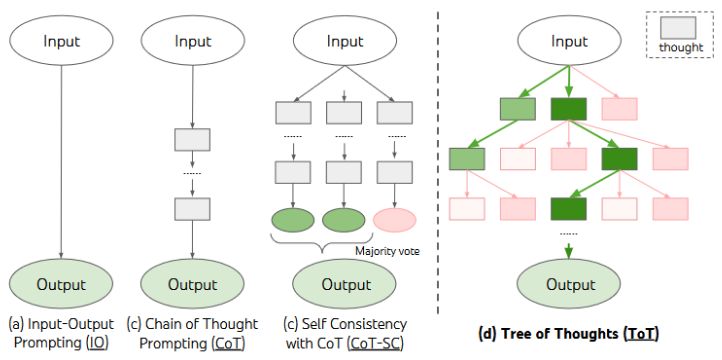
\includegraphics{figure/tot_vs_cot.png}\\
\citebutton{Yao et al., 2023}{https://arxiv.org/pdf/2305.10601.pdf}
\end{figure}

\vfill

\end{vbframe}

% ------------------------------------------------------------------------------


\begin{vbframe}{Tree-of-thought for creative writing}

\vfill

A step of deliberate search in a randomly picked Creative Writing task. Given the input, the LM samples five different plans, and then votes five times to decide which plan is best.
    
\begin{figure}
    \centering
    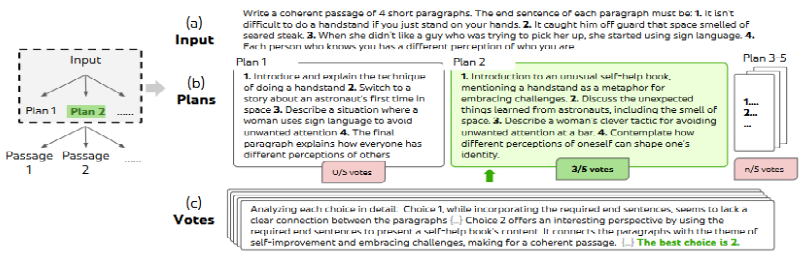
\includegraphics{figure/tot_creative_writing.png}\\
\citebutton{Yao et al., 2023}{https://arxiv.org/pdf/2305.10601.pdf}
\end{figure}

\vfill

\end{vbframe}

\begin{vbframe}{Tree-of-thought for creative writing (2)}

\vfill
    
\begin{figure}
\raisebox{0pt}[\height][\depth]{\hspace{-0.85cm}%
    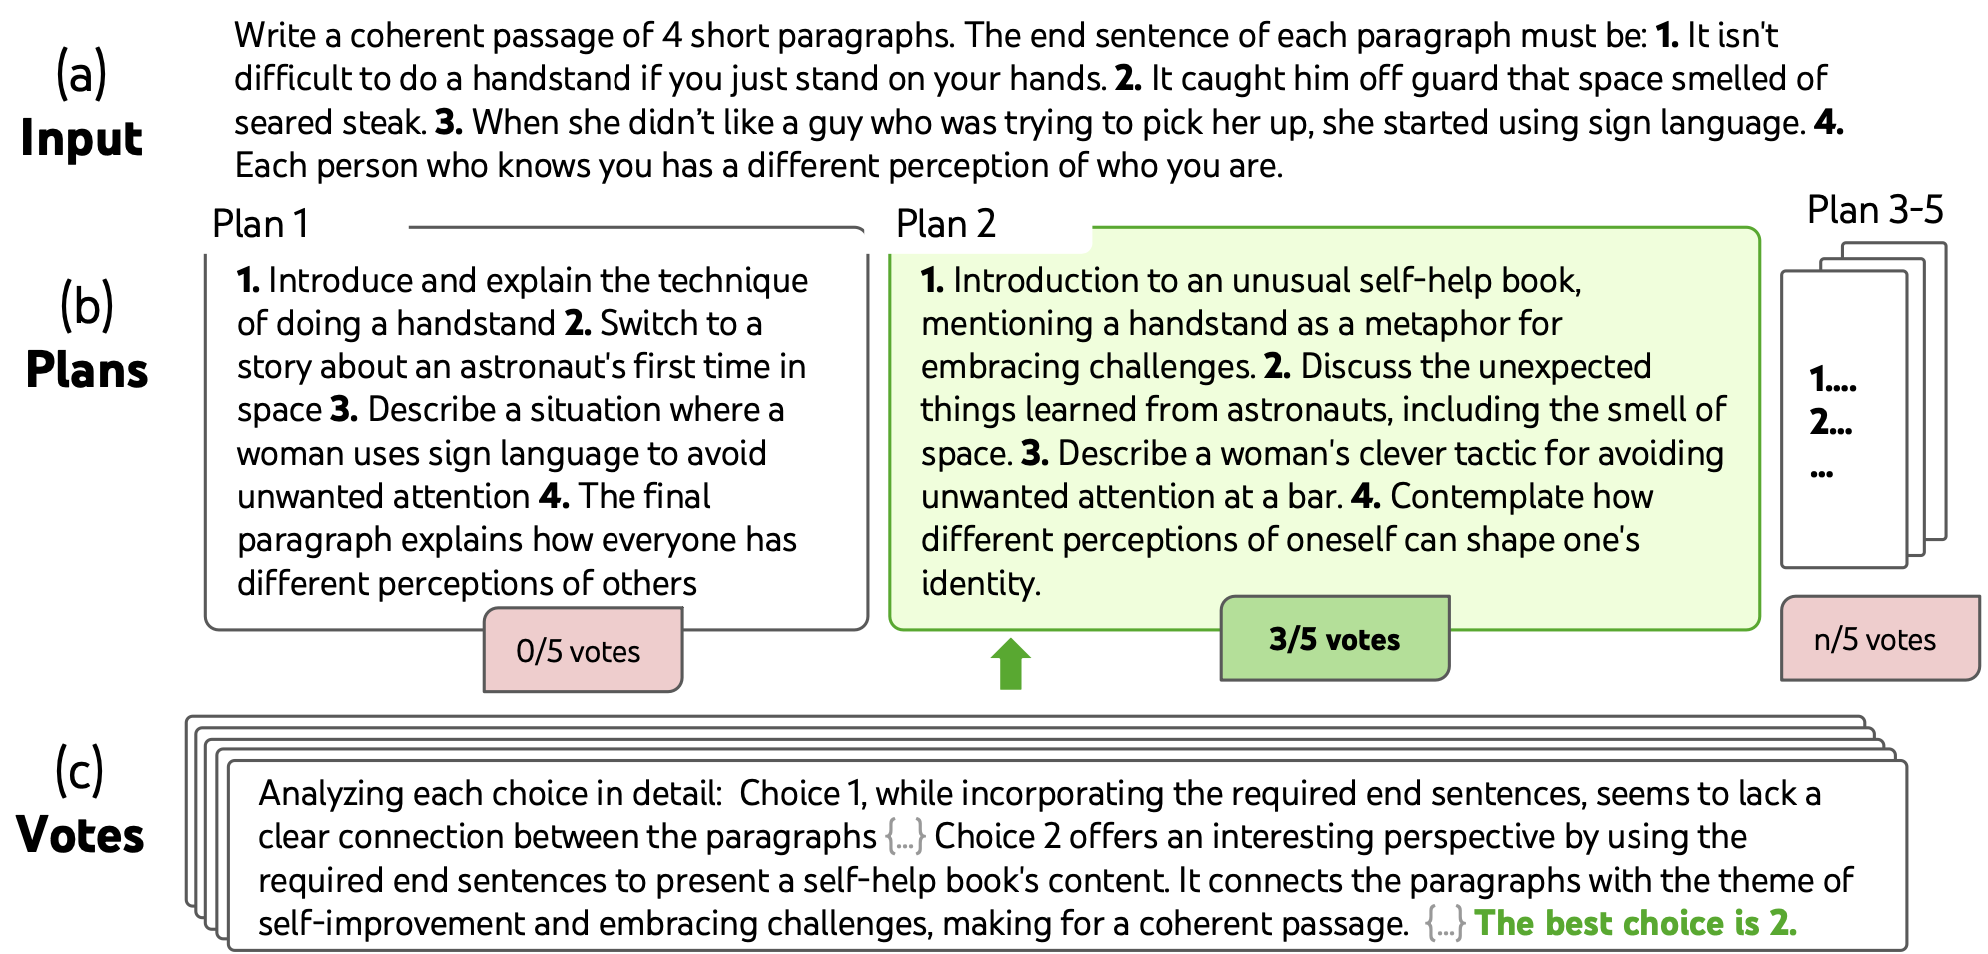
\includegraphics[width=1.15\textwidth]{figure/totcreativebig.png}
}
\end{figure}

\vfill

\end{vbframe}

% ------------------------------------------------------------------------------


\begin{frame}{\cotpfull: Error breakdown}

\vfill

\begin{itemize}
    \item 8\% calculator error
    \item 16\% symbol mapping error
    \item 22\% one missing step error
    \item rest: semantic issues, incoherent \cotp
\item Source: Stanford CS25: Beyond LLMs: Agents, Emergent
    Abilities, Intermediate-Guided Reasoning
\end{itemize}

\vfill

\end{frame}


\begin{frame}{\cotpfull: What could go wrong?}

\vfill

\begin{itemize}
    \item Decompose complex problems into a sequence of reasoning steps
    \item By describing the reasoning, interpretability is increased. It provides the possibility to observe where reasoning went wrong
    \item It is closer to how humans solve tasks using language
    \item Language models, if
given a well designed  chain-of-thought prompt, can
    solve problems they otherwise would not be able to solve.

\item \ques What could go wrong?
% no guarantee that the reasoning given is the reasoning employed
% is this true for humans?
% only one answer, but what happens if there is no good single answer?
% clearly a great thing for the examples given, but how
%    typical is this for what we need from language models?
%    -> go back to six examples that were blown up
%    inearlier slides
\end{itemize}

\vfill

\end{frame}

\begin{frame}{\cotpfull: Why does it work?}

\vfill

\begin{itemize}
    \item \ques Why does it work?
% make clear that reasoning is required
% make clear what kind o reasoning is rquirecd
% allocate additional compute
% LLMs are good at finding their own mistakes if
%    they look over there own output
\end{itemize}

\vfill

\end{frame}



\begin{frame}{\cotpfull: Why does it work?}

\vfill

\begin{itemize}
    \item \ques Do top-of-the-line LLMs use \cotpfull?
% show metricalfoot5.o.txt
% so this model uses chain of thought without chain of
%    thought prompting: how come?
% one possibility system prompt
% show system prompt
% e.g., "organize responses to flow well, not by source or citation
% another possibiley: standard training
% a third possibilty: new methdology, reasoning tokesn
\end{itemize}

\vfill

\end{frame}

\begin{frame}{Chain-of-Thought: Terminology}

\vfill

\begin{itemize}
    \item Shot = ``training example''
    \item few-shot prompting = few-shot learning
    \item The prompt ``think step by step'' by itself
    (without shots) is not \cotpfull.
    \item \cotpfull is defined as including shots.
    \item Chain-of-Thought is currently used as a general
    term to refer to the idea of LLMs using explicit
    reasoning steps to arrive at an answer.
    \item So the current usage of Chain-of-Thought is more
    general than \cotpfull.
\end{itemize}

\vfill

\end{frame}
\begin{frame}{Chain-of-Thought in OpenAI's o1}

\vfill

\begin{itemize}
    \item \citebutton{openai}{https://openai.com/index/learning-to-reason-with-llms/}
\item We are introducing OpenAI o1, a new large language
model trained with reinforcement learning to perform complex
reasoning. o1 thinks before it answers -- it can produce a long
internal chain of thought before responding to the user.
\item internal!
\end{itemize}

\vfill

\end{frame}

\begin{frame}{Generator-Verifier Gap (Noam Brown)}

\vfill

\begin{itemize}
    \item For many important problems, it is much easier to
    verify a solution than generating one.
    \item Chain-of-thought is expected to help for such
    problems with a generator-verifier gap.
    \item Problems with generator-verifier gap: Sudoku,
    doing math, programming
    \item Problems with less of a generator-verifier gap:
    knowledge questions (what is the capital of bhutan?),
    simple pattern matching (which language is this?)
    
\end{itemize}

\vfill

\end{frame}

\begin{frame}{Slido}

\vfill

\begin{itemize}
    \item 1313837 https://app.sli.do/event/dinLdZRBHw2fXo5R31C3Nt
    \item 1435969 https://app.sli.do/event/kWQDLpHa14256yiwxyCDr5
    \item 4039244 https://app.sli.do/event/ef5nQS8XmbhWAQDVk9CYQs
    \item 42248917 https://app.sli.do/event/5YwPZfoEFAibQ4DbFTzfj2
\end{itemize}

\vfill

\end{frame}



\endlecture
\end{document}
